\chapter{Исследовательский раздел}

%В данном разделе описано проведенное исследование производительности двух используемых в работе СУБД~---~Postgres и ClickHouse~---~при выполнении агрегационных запросов.

\section{Постановка исследования}
Целью исследования является сравнение времени выполнения агрегационных запросов с варьирующейся сложностью фильтрации данных в СУБД Postgres и ClickHouse. Исследование проводилось при количестве фильтров от 0, когда фильтрации не происходит, до 9. Даже на меньшем диапазоне разница в скорости обработки подобных запросов становится заметной.

Запросы выполнялись одновременно на разных серверах с одинаковыми характеристиками. Технические характеристики устройства, на котором выполнялось исследование~\cite{bib37}:
\begin{itemize}
	\item операционная система Ubuntu 22.04;
	\item 4 ГБ оперативной памяти;
	\item процессор с тактовой частотой 3.3 ГГц.
\end{itemize}

По результатам исследования была составлена сравнительная таблица и построен график зависимости времени выполнения запроса на агрегацию данных от количества применяемых к данным фильтров.

\section{Результаты исследования}
Результаты замеров времени выполнения (в мс) приведены в таблице~\ref{table:time}. Количество фильтров равное нулю означает, что фильтрация данных не производилась, то есть были получены все данные, хранимые в таблице. При замерах в таблице событий находилось 100 000 000 событий и было зарегистрировано 1000 клиентов.

\newpage

\begin{table}[]
\begin{center}
\caption{\label{table:time} Таблица сравнения времени выполнения агрегационных запросов с варьирующейся сложностью фильтрации данных в СУБД Postgres и ClickHouse}
\begin{tabular}{|c|l|l|}
\hline
\begin{tabular}[c]{@{}c@{}}Количество\\ фильтров\end{tabular} & \multicolumn{1}{c|}{\begin{tabular}[c]{@{}c@{}}Время выполнения\\ запроса в Postgres, мс\end{tabular}} & \multicolumn{1}{c|}{\begin{tabular}[c]{@{}c@{}}Время выполнения\\ запроса в СlickHouse, мс\end{tabular}} \\ \hline
0                                                             & 29325                                                                                                  & 385                                                                                                      \\ \hline
1                                                             & 28224                                                                                                  & 4322                                                                                                     \\ \hline
2                                                             & 51671                                                                                                  & 7966                                                                                                     \\ \hline
3                                                             & 76943                                                                                                  & 11947                                                                                                    \\ \hline
4                                                             & 94394                                                                                                  & 15959                                                                                                    \\ \hline
5                                                             & 117422                                                                                                 & 20059                                                                                                    \\ \hline
6                                                             & 143793                                                                                                 & 24127                                                                                                    \\ \hline
7                                                             & 171238                                                                                                 & 28409                                                                                                    \\ \hline
8                                                             & 193777                                                                                                 & 32350                                                                                                    \\ \hline
9                                                             & 210269                                                                                                 & 36201                                                                                                    \\ \hline
\end{tabular}
\end{center}
\end{table}

Зависимость времени выполнения агрегационных запросов от числа фильтров в СУБД Postgres и ClickHouse приведена на рисунке \ref{img:graph}.

\begin{table}[h!]
  \centering
  \begin{tabular}{p{1\linewidth}}
    \centering
    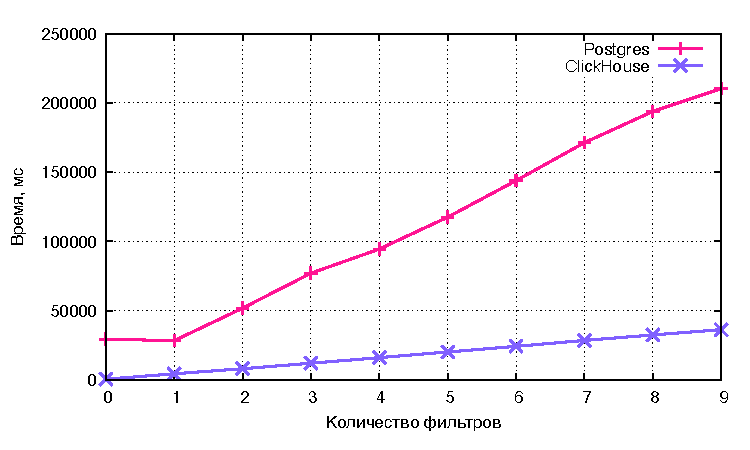
\includegraphics[width=1\linewidth]{./images/plot.pdf}
    \captionof{figure}{Сравнение времени выполнения агрегационных запросов в зависимости от числа фильтров в СУБД Postgres и ClickHouse}
    \label{img:graph}
  \end{tabular}
\end{table}

\section{Вывод}
В данном разделе было описано проведенное исследование производительности двух используемых в работе СУБД~---~Postgres и ClickHouse~---~при выполнении агрегационных запросов. Результаты исследования показывают, что агрегационные запросы более эффективно выполняются в ClickHouse. Без фильтрации запрос в ClickHouse выполняется быстрее запроса в Postgres в 76 раз. При 9 фильтрах это разница составляет 5 раз.

Также, зависимость скорости выполнения запроса от количества фильтров в ClickHouse практически линейная. При этом запрос в Postgres без фильтрации выполняется дольше, чем запрос с одним фильтром, что может быть связано с тем, что в первом случае необходимо было получить большее количество записей. 

Данное исследование показывает, что колоночные СУБД обрабатывают агрегационные запросы эффективнее строковых. Это объясняется тем, что агрегация чаще всего производится по значениям одного столбца. Доступ к данным одного столбца оптимизирован в СУБД колоночного типа в связи с особенностями хранения.
